\documentclass[twoside]{book}

% Packages required by doxygen
\usepackage{fixltx2e}
\usepackage{calc}
\usepackage{doxygen}
\usepackage[export]{adjustbox} % also loads graphicx
\usepackage{graphicx}
\usepackage[utf8]{inputenc}
\usepackage{makeidx}
\usepackage{multicol}
\usepackage{multirow}
\PassOptionsToPackage{warn}{textcomp}
\usepackage{textcomp}
\usepackage[nointegrals]{wasysym}
\usepackage[table]{xcolor}

% Font selection
\usepackage[T1]{fontenc}
\usepackage[scaled=.90]{helvet}
\usepackage{courier}
\usepackage{amssymb}
\usepackage{sectsty}
\renewcommand{\familydefault}{\sfdefault}
\allsectionsfont{%
  \fontseries{bc}\selectfont%
  \color{darkgray}%
}
\renewcommand{\DoxyLabelFont}{%
  \fontseries{bc}\selectfont%
  \color{darkgray}%
}
\newcommand{\+}{\discretionary{\mbox{\scriptsize$\hookleftarrow$}}{}{}}

% Page & text layout
\usepackage{geometry}
\geometry{%
  a4paper,%
  top=2.5cm,%
  bottom=2.5cm,%
  left=2.5cm,%
  right=2.5cm%
}
\tolerance=750
\hfuzz=15pt
\hbadness=750
\setlength{\emergencystretch}{15pt}
\setlength{\parindent}{0cm}
\setlength{\parskip}{3ex plus 2ex minus 2ex}
\makeatletter
\renewcommand{\paragraph}{%
  \@startsection{paragraph}{4}{0ex}{-1.0ex}{1.0ex}{%
    \normalfont\normalsize\bfseries\SS@parafont%
  }%
}
\renewcommand{\subparagraph}{%
  \@startsection{subparagraph}{5}{0ex}{-1.0ex}{1.0ex}{%
    \normalfont\normalsize\bfseries\SS@subparafont%
  }%
}
\makeatother

% Headers & footers
\usepackage{fancyhdr}
\pagestyle{fancyplain}
\fancyhead[LE]{\fancyplain{}{\bfseries\thepage}}
\fancyhead[CE]{\fancyplain{}{}}
\fancyhead[RE]{\fancyplain{}{\bfseries\leftmark}}
\fancyhead[LO]{\fancyplain{}{\bfseries\rightmark}}
\fancyhead[CO]{\fancyplain{}{}}
\fancyhead[RO]{\fancyplain{}{\bfseries\thepage}}
\fancyfoot[LE]{\fancyplain{}{}}
\fancyfoot[CE]{\fancyplain{}{}}
\fancyfoot[RE]{\fancyplain{}{\bfseries\scriptsize Generated by Doxygen }}
\fancyfoot[LO]{\fancyplain{}{\bfseries\scriptsize Generated by Doxygen }}
\fancyfoot[CO]{\fancyplain{}{}}
\fancyfoot[RO]{\fancyplain{}{}}
\renewcommand{\footrulewidth}{0.4pt}
\renewcommand{\chaptermark}[1]{%
  \markboth{#1}{}%
}
\renewcommand{\sectionmark}[1]{%
  \markright{\thesection\ #1}%
}

% Indices & bibliography
\usepackage{natbib}
\usepackage[titles]{tocloft}
\setcounter{tocdepth}{3}
\setcounter{secnumdepth}{5}
\makeindex

% Hyperlinks (required, but should be loaded last)
\usepackage{ifpdf}
\ifpdf
  \usepackage[pdftex,pagebackref=true]{hyperref}
\else
  \usepackage[ps2pdf,pagebackref=true]{hyperref}
\fi
\hypersetup{%
  colorlinks=true,%
  linkcolor=blue,%
  citecolor=blue,%
  unicode%
}

% Custom commands
\newcommand{\clearemptydoublepage}{%
  \newpage{\pagestyle{empty}\cleardoublepage}%
}

\usepackage{caption}
\captionsetup{labelsep=space,justification=centering,font={bf},singlelinecheck=off,skip=4pt,position=top}

%===== C O N T E N T S =====

\begin{document}

% Titlepage & ToC
\hypersetup{pageanchor=false,
             bookmarksnumbered=true,
             pdfencoding=unicode
            }
\pagenumbering{alph}
\begin{titlepage}
\vspace*{7cm}
\begin{center}%
{\Large Armanipulator-\/\+Firmware }\\
\vspace*{1cm}
{\large Generated by Doxygen 1.8.13}\\
\end{center}
\end{titlepage}
\clearemptydoublepage
\pagenumbering{roman}
\tableofcontents
\clearemptydoublepage
\pagenumbering{arabic}
\hypersetup{pageanchor=true}

%--- Begin generated contents ---
\chapter{Class Index}
\section{Class List}
Here are the classes, structs, unions and interfaces with brief descriptions\+:\begin{DoxyCompactList}
\item\contentsline{section}{\hyperlink{struct_controller_1_1arm__command}{Controller\+::arm\+\_\+command} }{\pageref{struct_controller_1_1arm__command}}{}
\item\contentsline{section}{\hyperlink{class_controller}{Controller} \\*The class-\/object used to interface between the serial interface and }{\pageref{class_controller}}{}
\item\contentsline{section}{\hyperlink{class_motor_config}{Motor\+Config} }{\pageref{class_motor_config}}{}
\item\contentsline{section}{\hyperlink{class_pinout}{Pinout} }{\pageref{class_pinout}}{}
\end{DoxyCompactList}

\chapter{File Index}
\section{File List}
Here is a list of all documented files with brief descriptions\+:\begin{DoxyCompactList}
\item\contentsline{section}{{\bfseries -\/\+E.\+d} }{\pageref{-_e_8d}}{}
\item\contentsline{section}{{\bfseries Controller.\+cpp} }{\pageref{_controller_8cpp}}{}
\item\contentsline{section}{\hyperlink{_controller_8h}{Controller.\+h} \\*Contains methods for controlling the motors and parsing input }{\pageref{_controller_8h}}{}
\item\contentsline{section}{{\bfseries cpu\+\_\+map.\+h} }{\pageref{cpu__map_8h}}{}
\item\contentsline{section}{{\bfseries sloeber.\+ino.\+cpp} }{\pageref{sloeber_8ino_8cpp}}{}
\item\contentsline{section}{{\bfseries spec.\+d} }{\pageref{spec_8d}}{}
\end{DoxyCompactList}

\chapter{Class Documentation}
\hypertarget{struct_controller_1_1arm__command}{}\section{Controller\+:\+:arm\+\_\+command Struct Reference}
\label{struct_controller_1_1arm__command}\index{Controller\+::arm\+\_\+command@{Controller\+::arm\+\_\+command}}


{\ttfamily \#include $<$Controller.\+h$>$}

\subsection*{Public Attributes}
\begin{DoxyCompactItemize}
\item 
\hyperlink{class_controller_a91a5751dd6920daf3b70814171b51767}{Controller\+::\+Arm\+\_\+\+Operation} \hyperlink{struct_controller_1_1arm__command_ac31649d9bb8a03e80a86a59bdfa0be75}{op}
\item 
double \hyperlink{struct_controller_1_1arm__command_a2e40c7e8947f625f1d39ac9568a1976a}{value}
\end{DoxyCompactItemize}


\subsection{Detailed Description}


Definition at line 49 of file Controller.\+h.



\subsection{Member Data Documentation}
\mbox{\Hypertarget{struct_controller_1_1arm__command_ac31649d9bb8a03e80a86a59bdfa0be75}\label{struct_controller_1_1arm__command_ac31649d9bb8a03e80a86a59bdfa0be75}} 
\index{Controller\+::arm\+\_\+command@{Controller\+::arm\+\_\+command}!op@{op}}
\index{op@{op}!Controller\+::arm\+\_\+command@{Controller\+::arm\+\_\+command}}
\subsubsection{\texorpdfstring{op}{op}}
{\footnotesize\ttfamily \hyperlink{class_controller_a91a5751dd6920daf3b70814171b51767}{Controller\+::\+Arm\+\_\+\+Operation} Controller\+::arm\+\_\+command\+::op}



Definition at line 50 of file Controller.\+h.



Referenced by Controller\+::execute\+Cmd(), Controller\+::parse\+Serial(), and Controller\+::print\+Exec().

\mbox{\Hypertarget{struct_controller_1_1arm__command_a2e40c7e8947f625f1d39ac9568a1976a}\label{struct_controller_1_1arm__command_a2e40c7e8947f625f1d39ac9568a1976a}} 
\index{Controller\+::arm\+\_\+command@{Controller\+::arm\+\_\+command}!value@{value}}
\index{value@{value}!Controller\+::arm\+\_\+command@{Controller\+::arm\+\_\+command}}
\subsubsection{\texorpdfstring{value}{value}}
{\footnotesize\ttfamily double Controller\+::arm\+\_\+command\+::value}



Definition at line 51 of file Controller.\+h.



Referenced by Controller\+::execute\+Cmd(), and Controller\+::parse\+Serial().



The documentation for this struct was generated from the following file\+:\begin{DoxyCompactItemize}
\item 
\hyperlink{_controller_8h}{Controller.\+h}\end{DoxyCompactItemize}

\hypertarget{class_controller}{}\section{Controller Class Reference}
\label{class_controller}\index{Controller@{Controller}}


The class-\/object used to interface between the serial interface and the stepper motor drivers.  




{\ttfamily \#include $<$Controller.\+h$>$}

\subsection*{Classes}
\begin{DoxyCompactItemize}
\item 
struct \hyperlink{struct_controller_1_1arm__command}{arm\+\_\+command}
\begin{DoxyCompactList}\small\item\em The structure used to define the overall instruction parsed from serial input. \end{DoxyCompactList}\end{DoxyCompactItemize}
\subsection*{Public Types}
\begin{DoxyCompactItemize}
\item 
enum \hyperlink{class_controller_a91a5751dd6920daf3b70814171b51767}{Arm\+\_\+\+Operation} \{ \newline
\hyperlink{class_controller_a91a5751dd6920daf3b70814171b51767a99ba9596fbe683c122b76174e7d40b8e}{R\+O\+T\+A\+TE}, 
\hyperlink{class_controller_a91a5751dd6920daf3b70814171b51767a41ed83326fd9ad04a2d24a228bc7a7ef}{G\+R\+AB}, 
\hyperlink{class_controller_a91a5751dd6920daf3b70814171b51767a1f9769fc0e78abe69b7a4ad5d573eb6c}{E\+X\+T\+E\+ND}, 
\hyperlink{class_controller_a91a5751dd6920daf3b70814171b51767a7d0e6ebddd2cb5dc5fb2100c018cc6d8}{M\+I\+C\+R\+O\+S\+T\+E\+PS}, 
\newline
\hyperlink{class_controller_a91a5751dd6920daf3b70814171b51767ae276bf8b30c8b606b54d8fb7d92c1ee6}{E\+R\+R\+OR}
 \}\begin{DoxyCompactList}\small\item\em Used to define common commands parsed by the arm. \end{DoxyCompactList}
\item 
enum \hyperlink{class_controller_aa94f1aea40982c422a43c1ee5aea0c49}{microsteps} \{ \newline
\hyperlink{class_controller_aa94f1aea40982c422a43c1ee5aea0c49a7c6a23455db73e86dcfafcb0025ac5dd}{H\+A\+LF}, 
\hyperlink{class_controller_aa94f1aea40982c422a43c1ee5aea0c49aa4e1dc476afca095736e176eb109dc11}{Q\+U\+A\+R\+T\+ER}, 
\hyperlink{class_controller_aa94f1aea40982c422a43c1ee5aea0c49a99f575098d1be025c224acc42fd921a0}{E\+I\+G\+TH}, 
\hyperlink{class_controller_aa94f1aea40982c422a43c1ee5aea0c49af214e4647ac3115a559b96a464219371}{S\+I\+X\+T\+E\+E\+N\+TH}, 
\newline
\hyperlink{class_controller_aa94f1aea40982c422a43c1ee5aea0c49aad17f41f310f462eb36ac9f6bac29b57}{T\+H\+I\+R\+T\+Y\+\_\+\+S\+E\+C\+O\+ND}
 \}
\item 
\mbox{\Hypertarget{class_controller_ab45ad0d63abd4b57021f13810fc856d3}\label{class_controller_ab45ad0d63abd4b57021f13810fc856d3}} 
typedef enum \hyperlink{class_controller_aa94f1aea40982c422a43c1ee5aea0c49}{Controller\+::microsteps} \hyperlink{class_controller_ab45ad0d63abd4b57021f13810fc856d3}{Microsteps}
\begin{DoxyCompactList}\small\item\em Used to placehold common Microstep configs for the motor drivers. \end{DoxyCompactList}\item 
typedef struct \hyperlink{struct_controller_1_1arm__command}{Controller\+::arm\+\_\+command} \hyperlink{class_controller_ac48cc99091f83f149fef8f17fd5d7e7f}{Arm\+\_\+\+Command}
\begin{DoxyCompactList}\small\item\em Type for the Arm\+\_\+\+Command Struct to allow easy definition. \end{DoxyCompactList}\end{DoxyCompactItemize}
\subsection*{Public Member Functions}
\begin{DoxyCompactItemize}
\item 
\mbox{\Hypertarget{class_controller_a95c56822d667e94b031451729ce069a9}\label{class_controller_a95c56822d667e94b031451729ce069a9}} 
\hyperlink{class_controller_a95c56822d667e94b031451729ce069a9}{Controller} ()
\begin{DoxyCompactList}\small\item\em Constructor for the controller object In this constructor, the motors are created on the heap, and then the motor pointer vars now point to the motors on the heap. current\+Cmd is not initialized, because it does not need to be pointed to at the minute. \end{DoxyCompactList}\item 
\mbox{\Hypertarget{class_controller_a0ab87934c4f7a266cfdb86e0f36bc1b5}\label{class_controller_a0ab87934c4f7a266cfdb86e0f36bc1b5}} 
virtual \hyperlink{class_controller_a0ab87934c4f7a266cfdb86e0f36bc1b5}{$\sim$\+Controller} ()
\begin{DoxyCompactList}\small\item\em Destructor for the controller object Has no purpose, therefore does nothing. \end{DoxyCompactList}\item 
void \hyperlink{class_controller_ad7583687bca402756ed9a4a8dc2e29ee}{parse\+Serial} (String rawinput)
\begin{DoxyCompactList}\small\item\em Translates Serial or Other Input into an Arm\+\_\+\+Command struct object This function will take the string input, and then parse based on the first character of the string. Parsing goes as follows\+: -\/\+Any commands related to rotation will start with an \textquotesingle{}r\textquotesingle{} or \textquotesingle{}R\textquotesingle{}, then followed by a double indicating revolutions -\/\+Any commands related to gripping will start with a \textquotesingle{}g\textquotesingle{} or \textquotesingle{}G\textquotesingle{}, then followed by a 0 or 1. Other values will trigger an exception -\/\+Any commands related to extending the arm will start with an \textquotesingle{}e\textquotesingle{} or \textquotesingle{}E\textquotesingle{}, then followed by a double indicating motor rotation. We will assert that the value is between -\/1 and 1 for now -\/\+Any unrecognized letter will return the E\+R\+R\+OR enum and 1 as the value. Serial should display an error message, or trigger an exception Once the command is selected, the remaining value is parsed as a double, and then pointed to in the Arm\+\_\+\+Command Pointer. \end{DoxyCompactList}\item 
void \hyperlink{class_controller_a8ad1d152a91997ab3825f32d2dcecfd4}{print\+Exec} ()
\begin{DoxyCompactList}\small\item\em Debug Function to test the parser Prints output in the serial connection based on the values in current\+Cmd. \end{DoxyCompactList}\item 
void \hyperlink{class_controller_ac1fc6cd2f507cc05e66a602e809c2446}{execute\+Cmd} ()
\begin{DoxyCompactList}\small\item\em Runs Commands based on data pointed to by current\+Cmd Uses the parsing rules defined by parse\+Serial and then do the respective action. \end{DoxyCompactList}\item 
\hyperlink{class_controller_ac48cc99091f83f149fef8f17fd5d7e7f}{Arm\+\_\+\+Command} $\ast$ \hyperlink{class_controller_af746c7701fda226720efe02890a308b2}{get\+Command} ()
\begin{DoxyCompactList}\small\item\em Getter method for the current\+Cmd pointer. \end{DoxyCompactList}\item 
void \hyperlink{class_controller_a951ce5ec5a6e653e9dd78b36351d80c5}{set\+Command} (\hyperlink{class_controller_ac48cc99091f83f149fef8f17fd5d7e7f}{Arm\+\_\+\+Command} $\ast$cmd)
\begin{DoxyCompactList}\small\item\em Setter method for the current\+Cmd pointer. \end{DoxyCompactList}\end{DoxyCompactItemize}


\subsection{Detailed Description}
The class-\/object used to interface between the serial interface and the stepper motor drivers. 

Definition at line 20 of file Controller.\+h.



\subsection{Member Typedef Documentation}
\mbox{\Hypertarget{class_controller_ac48cc99091f83f149fef8f17fd5d7e7f}\label{class_controller_ac48cc99091f83f149fef8f17fd5d7e7f}} 
\index{Controller@{Controller}!Arm\+\_\+\+Command@{Arm\+\_\+\+Command}}
\index{Arm\+\_\+\+Command@{Arm\+\_\+\+Command}!Controller@{Controller}}
\subsubsection{\texorpdfstring{Arm\+\_\+\+Command}{Arm\_Command}}
{\footnotesize\ttfamily \hyperlink{class_controller_ac48cc99091f83f149fef8f17fd5d7e7f}{Controller\+::\+Arm\+\_\+\+Command}}



Type for the Arm\+\_\+\+Command Struct to allow easy definition. 

\begin{DoxySeeAlso}{See also}
\hyperlink{struct_controller_1_1arm__command}{Controller\+::arm\+\_\+command} 
\end{DoxySeeAlso}


\subsection{Member Enumeration Documentation}
\mbox{\Hypertarget{class_controller_a91a5751dd6920daf3b70814171b51767}\label{class_controller_a91a5751dd6920daf3b70814171b51767}} 
\index{Controller@{Controller}!Arm\+\_\+\+Operation@{Arm\+\_\+\+Operation}}
\index{Arm\+\_\+\+Operation@{Arm\+\_\+\+Operation}!Controller@{Controller}}
\subsubsection{\texorpdfstring{Arm\+\_\+\+Operation}{Arm\_Operation}}
{\footnotesize\ttfamily enum \hyperlink{class_controller_a91a5751dd6920daf3b70814171b51767}{Controller\+::\+Arm\+\_\+\+Operation}}



Used to define common commands parsed by the arm. 

\begin{DoxyEnumFields}{Enumerator}
\raisebox{\heightof{T}}[0pt][0pt]{\index{R\+O\+T\+A\+TE@{R\+O\+T\+A\+TE}!Controller@{Controller}}\index{Controller@{Controller}!R\+O\+T\+A\+TE@{R\+O\+T\+A\+TE}}}\mbox{\Hypertarget{class_controller_a91a5751dd6920daf3b70814171b51767a99ba9596fbe683c122b76174e7d40b8e}\label{class_controller_a91a5751dd6920daf3b70814171b51767a99ba9596fbe683c122b76174e7d40b8e}} 
R\+O\+T\+A\+TE&Run the Wrist Rotation Motor \\
\hline

\raisebox{\heightof{T}}[0pt][0pt]{\index{G\+R\+AB@{G\+R\+AB}!Controller@{Controller}}\index{Controller@{Controller}!G\+R\+AB@{G\+R\+AB}}}\mbox{\Hypertarget{class_controller_a91a5751dd6920daf3b70814171b51767a41ed83326fd9ad04a2d24a228bc7a7ef}\label{class_controller_a91a5751dd6920daf3b70814171b51767a41ed83326fd9ad04a2d24a228bc7a7ef}} 
G\+R\+AB&Run the Grab motor \\
\hline

\raisebox{\heightof{T}}[0pt][0pt]{\index{E\+X\+T\+E\+ND@{E\+X\+T\+E\+ND}!Controller@{Controller}}\index{Controller@{Controller}!E\+X\+T\+E\+ND@{E\+X\+T\+E\+ND}}}\mbox{\Hypertarget{class_controller_a91a5751dd6920daf3b70814171b51767a1f9769fc0e78abe69b7a4ad5d573eb6c}\label{class_controller_a91a5751dd6920daf3b70814171b51767a1f9769fc0e78abe69b7a4ad5d573eb6c}} 
E\+X\+T\+E\+ND&Run the Arm Extender Motor \\
\hline

\raisebox{\heightof{T}}[0pt][0pt]{\index{M\+I\+C\+R\+O\+S\+T\+E\+PS@{M\+I\+C\+R\+O\+S\+T\+E\+PS}!Controller@{Controller}}\index{Controller@{Controller}!M\+I\+C\+R\+O\+S\+T\+E\+PS@{M\+I\+C\+R\+O\+S\+T\+E\+PS}}}\mbox{\Hypertarget{class_controller_a91a5751dd6920daf3b70814171b51767a7d0e6ebddd2cb5dc5fb2100c018cc6d8}\label{class_controller_a91a5751dd6920daf3b70814171b51767a7d0e6ebddd2cb5dc5fb2100c018cc6d8}} 
M\+I\+C\+R\+O\+S\+T\+E\+PS&Change the Microsteps for the driver \\
\hline

\raisebox{\heightof{T}}[0pt][0pt]{\index{E\+R\+R\+OR@{E\+R\+R\+OR}!Controller@{Controller}}\index{Controller@{Controller}!E\+R\+R\+OR@{E\+R\+R\+OR}}}\mbox{\Hypertarget{class_controller_a91a5751dd6920daf3b70814171b51767ae276bf8b30c8b606b54d8fb7d92c1ee6}\label{class_controller_a91a5751dd6920daf3b70814171b51767ae276bf8b30c8b606b54d8fb7d92c1ee6}} 
E\+R\+R\+OR&Default Error Placeholder \\
\hline

\end{DoxyEnumFields}


Definition at line 27 of file Controller.\+h.

\mbox{\Hypertarget{class_controller_aa94f1aea40982c422a43c1ee5aea0c49}\label{class_controller_aa94f1aea40982c422a43c1ee5aea0c49}} 
\index{Controller@{Controller}!microsteps@{microsteps}}
\index{microsteps@{microsteps}!Controller@{Controller}}
\subsubsection{\texorpdfstring{microsteps}{microsteps}}
{\footnotesize\ttfamily enum \hyperlink{class_controller_aa94f1aea40982c422a43c1ee5aea0c49}{Controller\+::microsteps}}

\begin{DoxyEnumFields}{Enumerator}
\raisebox{\heightof{T}}[0pt][0pt]{\index{H\+A\+LF@{H\+A\+LF}!Controller@{Controller}}\index{Controller@{Controller}!H\+A\+LF@{H\+A\+LF}}}\mbox{\Hypertarget{class_controller_aa94f1aea40982c422a43c1ee5aea0c49a7c6a23455db73e86dcfafcb0025ac5dd}\label{class_controller_aa94f1aea40982c422a43c1ee5aea0c49a7c6a23455db73e86dcfafcb0025ac5dd}} 
H\+A\+LF&1/2 Microstep Ratio \\
\hline

\raisebox{\heightof{T}}[0pt][0pt]{\index{Q\+U\+A\+R\+T\+ER@{Q\+U\+A\+R\+T\+ER}!Controller@{Controller}}\index{Controller@{Controller}!Q\+U\+A\+R\+T\+ER@{Q\+U\+A\+R\+T\+ER}}}\mbox{\Hypertarget{class_controller_aa94f1aea40982c422a43c1ee5aea0c49aa4e1dc476afca095736e176eb109dc11}\label{class_controller_aa94f1aea40982c422a43c1ee5aea0c49aa4e1dc476afca095736e176eb109dc11}} 
Q\+U\+A\+R\+T\+ER&1/4 Microstep Ratio \\
\hline

\raisebox{\heightof{T}}[0pt][0pt]{\index{E\+I\+G\+TH@{E\+I\+G\+TH}!Controller@{Controller}}\index{Controller@{Controller}!E\+I\+G\+TH@{E\+I\+G\+TH}}}\mbox{\Hypertarget{class_controller_aa94f1aea40982c422a43c1ee5aea0c49a99f575098d1be025c224acc42fd921a0}\label{class_controller_aa94f1aea40982c422a43c1ee5aea0c49a99f575098d1be025c224acc42fd921a0}} 
E\+I\+G\+TH&1/8 Microstep Ratio \\
\hline

\raisebox{\heightof{T}}[0pt][0pt]{\index{S\+I\+X\+T\+E\+E\+N\+TH@{S\+I\+X\+T\+E\+E\+N\+TH}!Controller@{Controller}}\index{Controller@{Controller}!S\+I\+X\+T\+E\+E\+N\+TH@{S\+I\+X\+T\+E\+E\+N\+TH}}}\mbox{\Hypertarget{class_controller_aa94f1aea40982c422a43c1ee5aea0c49af214e4647ac3115a559b96a464219371}\label{class_controller_aa94f1aea40982c422a43c1ee5aea0c49af214e4647ac3115a559b96a464219371}} 
S\+I\+X\+T\+E\+E\+N\+TH&1/16 Microstep Ratio \\
\hline

\raisebox{\heightof{T}}[0pt][0pt]{\index{T\+H\+I\+R\+T\+Y\+\_\+\+S\+E\+C\+O\+ND@{T\+H\+I\+R\+T\+Y\+\_\+\+S\+E\+C\+O\+ND}!Controller@{Controller}}\index{Controller@{Controller}!T\+H\+I\+R\+T\+Y\+\_\+\+S\+E\+C\+O\+ND@{T\+H\+I\+R\+T\+Y\+\_\+\+S\+E\+C\+O\+ND}}}\mbox{\Hypertarget{class_controller_aa94f1aea40982c422a43c1ee5aea0c49aad17f41f310f462eb36ac9f6bac29b57}\label{class_controller_aa94f1aea40982c422a43c1ee5aea0c49aad17f41f310f462eb36ac9f6bac29b57}} 
T\+H\+I\+R\+T\+Y\+\_\+\+S\+E\+C\+O\+ND&1/32 Microstep Ratio \\
\hline

\end{DoxyEnumFields}


Definition at line 38 of file Controller.\+h.



\subsection{Member Function Documentation}
\mbox{\Hypertarget{class_controller_ac1fc6cd2f507cc05e66a602e809c2446}\label{class_controller_ac1fc6cd2f507cc05e66a602e809c2446}} 
\index{Controller@{Controller}!execute\+Cmd@{execute\+Cmd}}
\index{execute\+Cmd@{execute\+Cmd}!Controller@{Controller}}
\subsubsection{\texorpdfstring{execute\+Cmd()}{executeCmd()}}
{\footnotesize\ttfamily Controller\+::execute\+Cmd (\begin{DoxyParamCaption}{ }\end{DoxyParamCaption})}



Runs Commands based on data pointed to by current\+Cmd Uses the parsing rules defined by parse\+Serial and then do the respective action. 

\begin{DoxySeeAlso}{See also}
\hyperlink{class_controller_ad7583687bca402756ed9a4a8dc2e29ee}{Controller\+::parse\+Serial} 
\end{DoxySeeAlso}


Definition at line 111 of file Controller.\+cpp.



References get\+Command(), Controller\+::arm\+\_\+command\+::op, and Controller\+::arm\+\_\+command\+::value.

Here is the call graph for this function\+:
\nopagebreak
\begin{figure}[H]
\begin{center}
\leavevmode
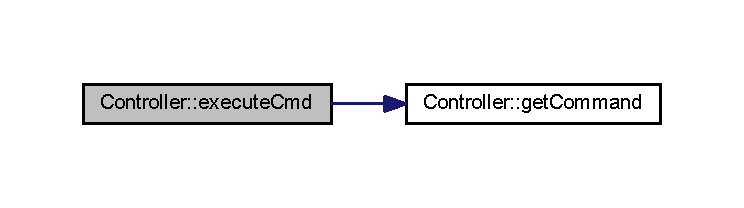
\includegraphics[width=350pt]{class_controller_ac1fc6cd2f507cc05e66a602e809c2446_cgraph}
\end{center}
\end{figure}
\mbox{\Hypertarget{class_controller_af746c7701fda226720efe02890a308b2}\label{class_controller_af746c7701fda226720efe02890a308b2}} 
\index{Controller@{Controller}!get\+Command@{get\+Command}}
\index{get\+Command@{get\+Command}!Controller@{Controller}}
\subsubsection{\texorpdfstring{get\+Command()}{getCommand()}}
{\footnotesize\ttfamily Controller\+::get\+Command (\begin{DoxyParamCaption}{ }\end{DoxyParamCaption})}



Getter method for the current\+Cmd pointer. 

\begin{DoxyReturn}{Returns}
Pointer to the Arm\+\_\+\+Command object of the pointer 
\end{DoxyReturn}


Definition at line 40 of file Controller.\+cpp.



Referenced by execute\+Cmd(), and print\+Exec().

\mbox{\Hypertarget{class_controller_ad7583687bca402756ed9a4a8dc2e29ee}\label{class_controller_ad7583687bca402756ed9a4a8dc2e29ee}} 
\index{Controller@{Controller}!parse\+Serial@{parse\+Serial}}
\index{parse\+Serial@{parse\+Serial}!Controller@{Controller}}
\subsubsection{\texorpdfstring{parse\+Serial()}{parseSerial()}}
{\footnotesize\ttfamily Controller\+::parse\+Serial (\begin{DoxyParamCaption}\item[{String}]{rawinput }\end{DoxyParamCaption})}



Translates Serial or Other Input into an Arm\+\_\+\+Command struct object This function will take the string input, and then parse based on the first character of the string. Parsing goes as follows\+: -\/\+Any commands related to rotation will start with an \textquotesingle{}r\textquotesingle{} or \textquotesingle{}R\textquotesingle{}, then followed by a double indicating revolutions -\/\+Any commands related to gripping will start with a \textquotesingle{}g\textquotesingle{} or \textquotesingle{}G\textquotesingle{}, then followed by a 0 or 1. Other values will trigger an exception -\/\+Any commands related to extending the arm will start with an \textquotesingle{}e\textquotesingle{} or \textquotesingle{}E\textquotesingle{}, then followed by a double indicating motor rotation. We will assert that the value is between -\/1 and 1 for now -\/\+Any unrecognized letter will return the E\+R\+R\+OR enum and 1 as the value. Serial should display an error message, or trigger an exception Once the command is selected, the remaining value is parsed as a double, and then pointed to in the Arm\+\_\+\+Command Pointer. 


\begin{DoxyParams}{Parameters}
{\em rawinput} & The input from Serial or other communication method \\
\hline
\end{DoxyParams}


Definition at line 49 of file Controller.\+cpp.



References Controller\+::arm\+\_\+command\+::op, and Controller\+::arm\+\_\+command\+::value.

\mbox{\Hypertarget{class_controller_a8ad1d152a91997ab3825f32d2dcecfd4}\label{class_controller_a8ad1d152a91997ab3825f32d2dcecfd4}} 
\index{Controller@{Controller}!print\+Exec@{print\+Exec}}
\index{print\+Exec@{print\+Exec}!Controller@{Controller}}
\subsubsection{\texorpdfstring{print\+Exec()}{printExec()}}
{\footnotesize\ttfamily Controller\+::print\+Exec (\begin{DoxyParamCaption}{ }\end{DoxyParamCaption})}



Debug Function to test the parser Prints output in the serial connection based on the values in current\+Cmd. 

\begin{DoxySeeAlso}{See also}
\hyperlink{class_controller_ad7583687bca402756ed9a4a8dc2e29ee}{Controller\+::parse\+Serial} 
\end{DoxySeeAlso}


Definition at line 81 of file Controller.\+cpp.



References get\+Command(), and Controller\+::arm\+\_\+command\+::op.

Here is the call graph for this function\+:
\nopagebreak
\begin{figure}[H]
\begin{center}
\leavevmode
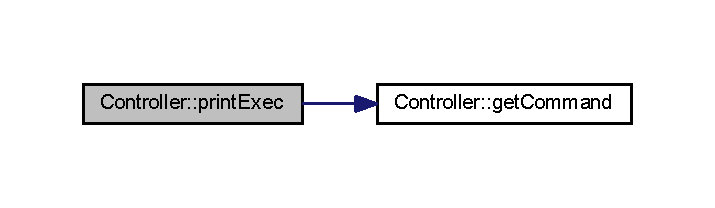
\includegraphics[width=343pt]{class_controller_a8ad1d152a91997ab3825f32d2dcecfd4_cgraph}
\end{center}
\end{figure}
\mbox{\Hypertarget{class_controller_a951ce5ec5a6e653e9dd78b36351d80c5}\label{class_controller_a951ce5ec5a6e653e9dd78b36351d80c5}} 
\index{Controller@{Controller}!set\+Command@{set\+Command}}
\index{set\+Command@{set\+Command}!Controller@{Controller}}
\subsubsection{\texorpdfstring{set\+Command()}{setCommand()}}
{\footnotesize\ttfamily Controller\+::set\+Command (\begin{DoxyParamCaption}\item[{\hyperlink{class_controller_ac48cc99091f83f149fef8f17fd5d7e7f}{Controller\+::\+Arm\+\_\+\+Command} $\ast$}]{cmd }\end{DoxyParamCaption})}



Setter method for the current\+Cmd pointer. 


\begin{DoxyParams}{Parameters}
{\em cmd} & The pointer to overwrite the current pointer of current\+Cmd \\
\hline
\end{DoxyParams}


Definition at line 44 of file Controller.\+cpp.



The documentation for this class was generated from the following files\+:\begin{DoxyCompactItemize}
\item 
\hyperlink{_controller_8h}{Controller.\+h}\item 
Controller.\+cpp\end{DoxyCompactItemize}

\hypertarget{class_motor_config}{}\section{Motor\+Config Class Reference}
\label{class_motor_config}\index{Motor\+Config@{Motor\+Config}}


{\ttfamily \#include $<$cpu\+\_\+map.\+h$>$}

\subsection*{Static Public Attributes}
\begin{DoxyCompactItemize}
\item 
static const short \hyperlink{class_motor_config_a7c9848ce827ad884f69001c8517178a7}{M\+O\+T\+O\+R\+\_\+\+S\+T\+E\+PS} = 200
\item 
static const short \hyperlink{class_motor_config_a9671c799866d18d9bec915fc6b55f7b8}{M\+I\+C\+R\+O\+S\+T\+E\+PS} = 1
\item 
static const short \hyperlink{class_motor_config_abe3fe3efcce60033bf58a93fda1c1011}{M\+O\+T\+O\+R\+\_\+\+R\+PM} = 120
\end{DoxyCompactItemize}


\subsection{Detailed Description}


Definition at line 46 of file cpu\+\_\+map.\+h.



\subsection{Member Data Documentation}
\mbox{\Hypertarget{class_motor_config_a9671c799866d18d9bec915fc6b55f7b8}\label{class_motor_config_a9671c799866d18d9bec915fc6b55f7b8}} 
\index{Motor\+Config@{Motor\+Config}!M\+I\+C\+R\+O\+S\+T\+E\+PS@{M\+I\+C\+R\+O\+S\+T\+E\+PS}}
\index{M\+I\+C\+R\+O\+S\+T\+E\+PS@{M\+I\+C\+R\+O\+S\+T\+E\+PS}!Motor\+Config@{Motor\+Config}}
\subsubsection{\texorpdfstring{M\+I\+C\+R\+O\+S\+T\+E\+PS}{MICROSTEPS}}
{\footnotesize\ttfamily const short Motor\+Config\+::\+M\+I\+C\+R\+O\+S\+T\+E\+PS = 1\hspace{0.3cm}{\ttfamily [static]}}



Definition at line 56 of file cpu\+\_\+map.\+h.



Referenced by Controller\+::\+Controller().

\mbox{\Hypertarget{class_motor_config_abe3fe3efcce60033bf58a93fda1c1011}\label{class_motor_config_abe3fe3efcce60033bf58a93fda1c1011}} 
\index{Motor\+Config@{Motor\+Config}!M\+O\+T\+O\+R\+\_\+\+R\+PM@{M\+O\+T\+O\+R\+\_\+\+R\+PM}}
\index{M\+O\+T\+O\+R\+\_\+\+R\+PM@{M\+O\+T\+O\+R\+\_\+\+R\+PM}!Motor\+Config@{Motor\+Config}}
\subsubsection{\texorpdfstring{M\+O\+T\+O\+R\+\_\+\+R\+PM}{MOTOR\_RPM}}
{\footnotesize\ttfamily const short Motor\+Config\+::\+M\+O\+T\+O\+R\+\_\+\+R\+PM = 120\hspace{0.3cm}{\ttfamily [static]}}



Definition at line 61 of file cpu\+\_\+map.\+h.



Referenced by Controller\+::\+Controller().

\mbox{\Hypertarget{class_motor_config_a7c9848ce827ad884f69001c8517178a7}\label{class_motor_config_a7c9848ce827ad884f69001c8517178a7}} 
\index{Motor\+Config@{Motor\+Config}!M\+O\+T\+O\+R\+\_\+\+S\+T\+E\+PS@{M\+O\+T\+O\+R\+\_\+\+S\+T\+E\+PS}}
\index{M\+O\+T\+O\+R\+\_\+\+S\+T\+E\+PS@{M\+O\+T\+O\+R\+\_\+\+S\+T\+E\+PS}!Motor\+Config@{Motor\+Config}}
\subsubsection{\texorpdfstring{M\+O\+T\+O\+R\+\_\+\+S\+T\+E\+PS}{MOTOR\_STEPS}}
{\footnotesize\ttfamily const short Motor\+Config\+::\+M\+O\+T\+O\+R\+\_\+\+S\+T\+E\+PS = 200\hspace{0.3cm}{\ttfamily [static]}}



Definition at line 51 of file cpu\+\_\+map.\+h.



Referenced by Controller\+::\+Controller().



The documentation for this class was generated from the following file\+:\begin{DoxyCompactItemize}
\item 
\hyperlink{cpu__map_8h}{cpu\+\_\+map.\+h}\end{DoxyCompactItemize}

\hypertarget{class_pinout}{}\section{Pinout Class Reference}
\label{class_pinout}\index{Pinout@{Pinout}}


{\ttfamily \#include $<$cpu\+\_\+map.\+h$>$}

\subsection*{Static Public Attributes}
\begin{DoxyCompactItemize}
\item 
static const short \hyperlink{class_pinout_a5f15f2424dc98ebf66f74063798ae28e}{W\+R\+I\+S\+T\+\_\+\+R\+O\+T\+\_\+\+S\+T\+EP} = 2
\item 
static const short \hyperlink{class_pinout_a2bdfc2d0feb1763149886acaab1a0419}{W\+R\+I\+S\+T\+\_\+\+R\+O\+T\+\_\+\+D\+IR} = 3
\item 
static const short \hyperlink{class_pinout_a034e6fd901a557f17809260288ea4740}{G\+R\+I\+P\+\_\+\+S\+T\+EP} = 4
\item 
static const short \hyperlink{class_pinout_a49466f79a0074d31c74885c4876693de}{G\+R\+I\+P\+\_\+\+D\+IR} = 5
\item 
static const short \hyperlink{class_pinout_a69dd96e739859d5cc64e477ca844276b}{E\+X\+T\+E\+N\+D\+\_\+\+S\+T\+EP} = 6
\item 
static const short \hyperlink{class_pinout_a361ce1c43bf6c143f2ae3e85ba0d5e25}{E\+X\+T\+E\+N\+D\+\_\+\+D\+IR} = 7
\end{DoxyCompactItemize}


\subsection{Detailed Description}


Definition at line 11 of file cpu\+\_\+map.\+h.



\subsection{Member Data Documentation}
\mbox{\Hypertarget{class_pinout_a361ce1c43bf6c143f2ae3e85ba0d5e25}\label{class_pinout_a361ce1c43bf6c143f2ae3e85ba0d5e25}} 
\index{Pinout@{Pinout}!E\+X\+T\+E\+N\+D\+\_\+\+D\+IR@{E\+X\+T\+E\+N\+D\+\_\+\+D\+IR}}
\index{E\+X\+T\+E\+N\+D\+\_\+\+D\+IR@{E\+X\+T\+E\+N\+D\+\_\+\+D\+IR}!Pinout@{Pinout}}
\subsubsection{\texorpdfstring{E\+X\+T\+E\+N\+D\+\_\+\+D\+IR}{EXTEND\_DIR}}
{\footnotesize\ttfamily const short Pinout\+::\+E\+X\+T\+E\+N\+D\+\_\+\+D\+IR = 7\hspace{0.3cm}{\ttfamily [static]}}



Definition at line 42 of file cpu\+\_\+map.\+h.



Referenced by Controller\+::\+Controller().

\mbox{\Hypertarget{class_pinout_a69dd96e739859d5cc64e477ca844276b}\label{class_pinout_a69dd96e739859d5cc64e477ca844276b}} 
\index{Pinout@{Pinout}!E\+X\+T\+E\+N\+D\+\_\+\+S\+T\+EP@{E\+X\+T\+E\+N\+D\+\_\+\+S\+T\+EP}}
\index{E\+X\+T\+E\+N\+D\+\_\+\+S\+T\+EP@{E\+X\+T\+E\+N\+D\+\_\+\+S\+T\+EP}!Pinout@{Pinout}}
\subsubsection{\texorpdfstring{E\+X\+T\+E\+N\+D\+\_\+\+S\+T\+EP}{EXTEND\_STEP}}
{\footnotesize\ttfamily const short Pinout\+::\+E\+X\+T\+E\+N\+D\+\_\+\+S\+T\+EP = 6\hspace{0.3cm}{\ttfamily [static]}}



Definition at line 36 of file cpu\+\_\+map.\+h.



Referenced by Controller\+::\+Controller().

\mbox{\Hypertarget{class_pinout_a49466f79a0074d31c74885c4876693de}\label{class_pinout_a49466f79a0074d31c74885c4876693de}} 
\index{Pinout@{Pinout}!G\+R\+I\+P\+\_\+\+D\+IR@{G\+R\+I\+P\+\_\+\+D\+IR}}
\index{G\+R\+I\+P\+\_\+\+D\+IR@{G\+R\+I\+P\+\_\+\+D\+IR}!Pinout@{Pinout}}
\subsubsection{\texorpdfstring{G\+R\+I\+P\+\_\+\+D\+IR}{GRIP\_DIR}}
{\footnotesize\ttfamily const short Pinout\+::\+G\+R\+I\+P\+\_\+\+D\+IR = 5\hspace{0.3cm}{\ttfamily [static]}}



Definition at line 32 of file cpu\+\_\+map.\+h.



Referenced by Controller\+::\+Controller().

\mbox{\Hypertarget{class_pinout_a034e6fd901a557f17809260288ea4740}\label{class_pinout_a034e6fd901a557f17809260288ea4740}} 
\index{Pinout@{Pinout}!G\+R\+I\+P\+\_\+\+S\+T\+EP@{G\+R\+I\+P\+\_\+\+S\+T\+EP}}
\index{G\+R\+I\+P\+\_\+\+S\+T\+EP@{G\+R\+I\+P\+\_\+\+S\+T\+EP}!Pinout@{Pinout}}
\subsubsection{\texorpdfstring{G\+R\+I\+P\+\_\+\+S\+T\+EP}{GRIP\_STEP}}
{\footnotesize\ttfamily const short Pinout\+::\+G\+R\+I\+P\+\_\+\+S\+T\+EP = 4\hspace{0.3cm}{\ttfamily [static]}}



Definition at line 27 of file cpu\+\_\+map.\+h.



Referenced by Controller\+::\+Controller().

\mbox{\Hypertarget{class_pinout_a2bdfc2d0feb1763149886acaab1a0419}\label{class_pinout_a2bdfc2d0feb1763149886acaab1a0419}} 
\index{Pinout@{Pinout}!W\+R\+I\+S\+T\+\_\+\+R\+O\+T\+\_\+\+D\+IR@{W\+R\+I\+S\+T\+\_\+\+R\+O\+T\+\_\+\+D\+IR}}
\index{W\+R\+I\+S\+T\+\_\+\+R\+O\+T\+\_\+\+D\+IR@{W\+R\+I\+S\+T\+\_\+\+R\+O\+T\+\_\+\+D\+IR}!Pinout@{Pinout}}
\subsubsection{\texorpdfstring{W\+R\+I\+S\+T\+\_\+\+R\+O\+T\+\_\+\+D\+IR}{WRIST\_ROT\_DIR}}
{\footnotesize\ttfamily const short Pinout\+::\+W\+R\+I\+S\+T\+\_\+\+R\+O\+T\+\_\+\+D\+IR = 3\hspace{0.3cm}{\ttfamily [static]}}



Definition at line 22 of file cpu\+\_\+map.\+h.



Referenced by Controller\+::\+Controller().

\mbox{\Hypertarget{class_pinout_a5f15f2424dc98ebf66f74063798ae28e}\label{class_pinout_a5f15f2424dc98ebf66f74063798ae28e}} 
\index{Pinout@{Pinout}!W\+R\+I\+S\+T\+\_\+\+R\+O\+T\+\_\+\+S\+T\+EP@{W\+R\+I\+S\+T\+\_\+\+R\+O\+T\+\_\+\+S\+T\+EP}}
\index{W\+R\+I\+S\+T\+\_\+\+R\+O\+T\+\_\+\+S\+T\+EP@{W\+R\+I\+S\+T\+\_\+\+R\+O\+T\+\_\+\+S\+T\+EP}!Pinout@{Pinout}}
\subsubsection{\texorpdfstring{W\+R\+I\+S\+T\+\_\+\+R\+O\+T\+\_\+\+S\+T\+EP}{WRIST\_ROT\_STEP}}
{\footnotesize\ttfamily const short Pinout\+::\+W\+R\+I\+S\+T\+\_\+\+R\+O\+T\+\_\+\+S\+T\+EP = 2\hspace{0.3cm}{\ttfamily [static]}}



Definition at line 17 of file cpu\+\_\+map.\+h.



Referenced by Controller\+::\+Controller().



The documentation for this class was generated from the following file\+:\begin{DoxyCompactItemize}
\item 
\hyperlink{cpu__map_8h}{cpu\+\_\+map.\+h}\end{DoxyCompactItemize}

\chapter{File Documentation}
\hypertarget{-_e_8d}{}\section{-\/E.d File Reference}
\label{-_e_8d}\index{-\/\+E.\+d@{-\/\+E.\+d}}

\hypertarget{_controller_8cpp}{}\section{Controller.\+cpp File Reference}
\label{_controller_8cpp}\index{Controller.\+cpp@{Controller.\+cpp}}
{\ttfamily \#include \char`\"{}Controller.\+h\char`\"{}}\newline
{\ttfamily \#include \char`\"{}cpu\+\_\+map.\+h\char`\"{}}\newline
Include dependency graph for Controller.\+cpp\+:\nopagebreak
\begin{figure}[H]
\begin{center}
\leavevmode
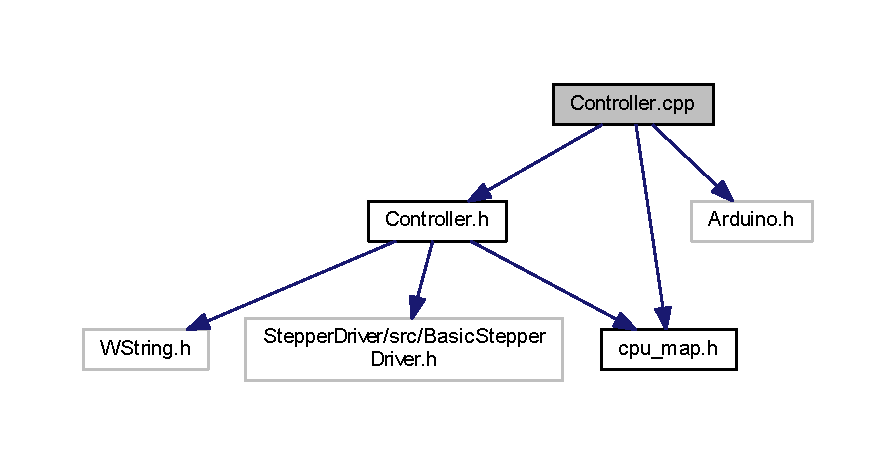
\includegraphics[width=350pt]{_controller_8cpp__incl}
\end{center}
\end{figure}
\subsection*{Variables}
\begin{DoxyCompactItemize}
\item 
\hyperlink{class_controller_ac48cc99091f83f149fef8f17fd5d7e7f}{Controller\+::\+Arm\+\_\+\+Command} $\ast$ \hyperlink{_controller_8cpp_add17797b9c4282f6e91f6d2f0a58a6cc}{current\+Cmd}
\item 
Basic\+Stepper\+Driver $\ast$ \hyperlink{_controller_8cpp_a42b5f2c17e34717e264a99e17a35a445}{rotate\+Driver}
\item 
Basic\+Stepper\+Driver $\ast$ \hyperlink{_controller_8cpp_a84ed43e9619bc0d37bfcad2d1c74333d}{grab\+Driver}
\item 
Basic\+Stepper\+Driver $\ast$ \hyperlink{_controller_8cpp_a64545030bf193d46b9f256ba134a750d}{extend\+Driver}
\end{DoxyCompactItemize}


\subsection{Variable Documentation}
\mbox{\Hypertarget{_controller_8cpp_add17797b9c4282f6e91f6d2f0a58a6cc}\label{_controller_8cpp_add17797b9c4282f6e91f6d2f0a58a6cc}} 
\index{Controller.\+cpp@{Controller.\+cpp}!current\+Cmd@{current\+Cmd}}
\index{current\+Cmd@{current\+Cmd}!Controller.\+cpp@{Controller.\+cpp}}
\subsubsection{\texorpdfstring{current\+Cmd}{currentCmd}}
{\footnotesize\ttfamily \hyperlink{class_controller_ac48cc99091f83f149fef8f17fd5d7e7f}{Controller\+::\+Arm\+\_\+\+Command}$\ast$ current\+Cmd}



Definition at line 12 of file Controller.\+cpp.

\mbox{\Hypertarget{_controller_8cpp_a64545030bf193d46b9f256ba134a750d}\label{_controller_8cpp_a64545030bf193d46b9f256ba134a750d}} 
\index{Controller.\+cpp@{Controller.\+cpp}!extend\+Driver@{extend\+Driver}}
\index{extend\+Driver@{extend\+Driver}!Controller.\+cpp@{Controller.\+cpp}}
\subsubsection{\texorpdfstring{extend\+Driver}{extendDriver}}
{\footnotesize\ttfamily Basic\+Stepper\+Driver$\ast$ extend\+Driver}



Definition at line 15 of file Controller.\+cpp.

\mbox{\Hypertarget{_controller_8cpp_a84ed43e9619bc0d37bfcad2d1c74333d}\label{_controller_8cpp_a84ed43e9619bc0d37bfcad2d1c74333d}} 
\index{Controller.\+cpp@{Controller.\+cpp}!grab\+Driver@{grab\+Driver}}
\index{grab\+Driver@{grab\+Driver}!Controller.\+cpp@{Controller.\+cpp}}
\subsubsection{\texorpdfstring{grab\+Driver}{grabDriver}}
{\footnotesize\ttfamily Basic\+Stepper\+Driver$\ast$ grab\+Driver}



Definition at line 14 of file Controller.\+cpp.

\mbox{\Hypertarget{_controller_8cpp_a42b5f2c17e34717e264a99e17a35a445}\label{_controller_8cpp_a42b5f2c17e34717e264a99e17a35a445}} 
\index{Controller.\+cpp@{Controller.\+cpp}!rotate\+Driver@{rotate\+Driver}}
\index{rotate\+Driver@{rotate\+Driver}!Controller.\+cpp@{Controller.\+cpp}}
\subsubsection{\texorpdfstring{rotate\+Driver}{rotateDriver}}
{\footnotesize\ttfamily Basic\+Stepper\+Driver$\ast$ rotate\+Driver}



Definition at line 13 of file Controller.\+cpp.


\hypertarget{_controller_8h}{}\section{Controller.\+h File Reference}
\label{_controller_8h}\index{Controller.\+h@{Controller.\+h}}


Contains methods for controlling the motors and parsing input.  


{\ttfamily \#include $<$W\+String.\+h$>$}\newline
{\ttfamily \#include \char`\"{}Stepper\+Driver/src/\+Basic\+Stepper\+Driver.\+h\char`\"{}}\newline
{\ttfamily \#include \char`\"{}cpu\+\_\+map.\+h\char`\"{}}\newline
Include dependency graph for Controller.\+h\+:
\nopagebreak
\begin{figure}[H]
\begin{center}
\leavevmode
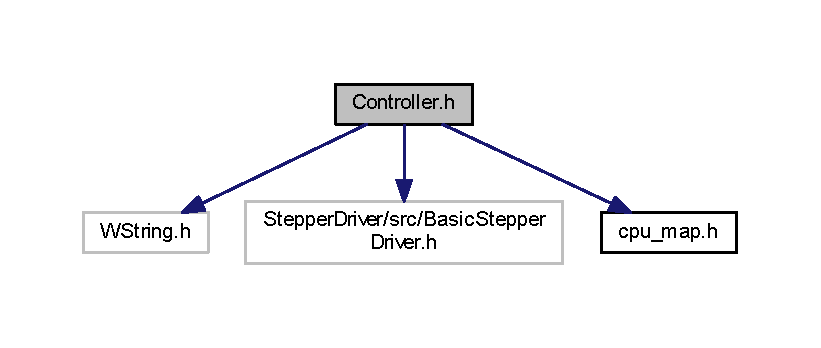
\includegraphics[width=350pt]{_controller_8h__incl}
\end{center}
\end{figure}
This graph shows which files directly or indirectly include this file\+:
\nopagebreak
\begin{figure}[H]
\begin{center}
\leavevmode
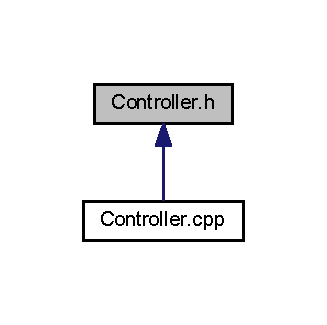
\includegraphics[width=157pt]{_controller_8h__dep__incl}
\end{center}
\end{figure}
\subsection*{Classes}
\begin{DoxyCompactItemize}
\item 
class \hyperlink{class_controller}{Controller}
\begin{DoxyCompactList}\small\item\em The class-\/object used to interface between the serial interface and the stepper motor drivers. \end{DoxyCompactList}\item 
struct \hyperlink{struct_controller_1_1arm__command}{Controller\+::arm\+\_\+command}
\begin{DoxyCompactList}\small\item\em The structure used to define the overall instruction parsed from serial input. \end{DoxyCompactList}\end{DoxyCompactItemize}


\subsection{Detailed Description}
Contains methods for controlling the motors and parsing input. 


\hypertarget{cpu__map_8h}{}\section{cpu\+\_\+map.\+h File Reference}
\label{cpu__map_8h}\index{cpu\+\_\+map.\+h@{cpu\+\_\+map.\+h}}
This graph shows which files directly or indirectly include this file\+:\nopagebreak
\begin{figure}[H]
\begin{center}
\leavevmode
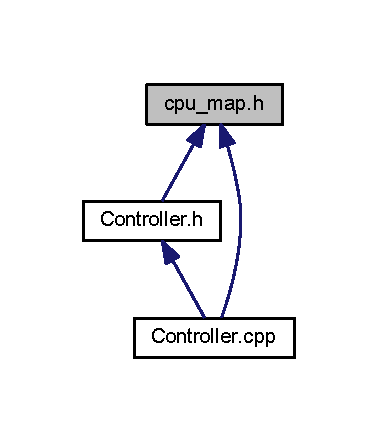
\includegraphics[width=182pt]{cpu__map_8h__dep__incl}
\end{center}
\end{figure}
\subsection*{Classes}
\begin{DoxyCompactItemize}
\item 
class \hyperlink{class_pinout}{Pinout}
\item 
class \hyperlink{class_motor_config}{Motor\+Config}
\end{DoxyCompactItemize}

\hypertarget{sloeber_8ino_8cpp}{}\section{sloeber.\+ino.\+cpp File Reference}
\label{sloeber_8ino_8cpp}\index{sloeber.\+ino.\+cpp@{sloeber.\+ino.\+cpp}}

\hypertarget{spec_8d}{}\section{spec.\+d File Reference}
\label{spec_8d}\index{spec.\+d@{spec.\+d}}

%--- End generated contents ---

% Index
\backmatter
\newpage
\phantomsection
\clearemptydoublepage
\addcontentsline{toc}{chapter}{Index}
\printindex

\end{document}
